%%%%%%%%%%%%%%%%%%%%%%%%%%%%%%%%%%%%%%%%%%%%%%%%%%%%%%%%%%%%%%%%%%%%%%%%%%%%%%%%%%%%%%%%%%%%%%%%%%%%%%%%%%%%%%%%%%%%%%%%%%%%%%%%%%%%%%%%%%%%%%%%%%%%%%%%%%%
% This is just an example/guide for you to refer to when submitting manuscripts to Frontiers, it is not mandatory to use Frontiers .cls files nor frontiers.tex  %
% This will only generate the Manuscript, the final article will be typeset by Frontiers after acceptance.   
%                                              %
%                                                                                                                                                         %
% When submitting your files, remember to upload this *tex file, the pdf generated with it, the *bib file (if bibliography is not within the *tex) and all the figures.
%%%%%%%%%%%%%%%%%%%%%%%%%%%%%%%%%%%%%%%%%%%%%%%%%%%%%%%%%%%%%%%%%%%%%%%%%%%%%%%%%%%%%%%%%%%%%%%%%%%%%%%%%%%%%%%%%%%%%%%%%%%%%%%%%%%%%%%%%%%%%%%%%%%%%%%%%%%

%%% Version 3.4 Generated 2018/06/15 %%%
%%% You will need to have the following packages installed: datetime, fmtcount, etoolbox, fcprefix, which are normally inlcuded in WinEdt. %%%
%%% In http://www.ctan.org/ you can find the packages and how to install them, if necessary. %%%
%%%  NB logo1.jpg is required in the path in order to correctly compile front page header %%%

\documentclass[utf8]{frontiersSCNS} % for Science, Engineering and Humanities and Social Sciences articles
%\documentclass[utf8]{frontiersHLTH} % for Health articles
%\documentclass[utf8]{frontiersFPHY} % for Physics and Applied Mathematics and Statistics articles

%\setcitestyle{square} % for Physics and Applied Mathematics and Statistics articles
\usepackage{url,hyperref,lineno,microtype,subcaption}
\usepackage[onehalfspacing]{setspace}

\linenumbers


% Leave a blank line between paragraphs instead of using \\


\def\keyFont{\fontsize{8}{11}\helveticabold }
\def\firstAuthorLast{Treder} %use et al only if is more than 1 author
\def\Authors{Matthias S. Treder}
% Affiliations should be keyed to the author's name with superscript numbers and be listed as follows: Laboratory, Institute, Department, Organization, City, State abbreviation (USA, Canada, Australia), and Country (without detailed address information such as city zip codes or street names).
% If one of the authors has a change of address, list the new address below the correspondence details using a superscript symbol and use the same symbol to indicate the author in the author list.
\def\Address{School of Computer Science \& Informatics, Cardiff University, Cardiff, UK}
% The Corresponding Author should be marked with an asterisk
% Provide the exact contact address (this time including street name and city zip code) and email of the corresponding author
\def\corrAuthor{Corresponding Author}

\def\corrEmail{trederm@cardiff.ac.uk}

%%% --- added by Matthias ---
\usepackage{tabularx}  % controls the table width
\usepackage{prettyref}
\usepackage{amsmath}
\usepackage{xcolor}
\usepackage{bbm}    % for 1 as a vector

\newtheorem{theorem}{Theorem}

% Math symbols
\newcommand{\al}{\boldsymbol{\alpha}}
\newcommand{\m}{\mathbf{m}}
\newcommand{\mbar}{\overline{\m}}
\newcommand{\mm}[1]{\m_{#1}}
\newcommand{\w}{\mathbf{w}}
\newcommand{\x}{\mathbf{x}}
\newcommand{\y}{\mathbf{y}}
\newcommand{\C}{\mathbf{C}}
\newcommand{\cov}{\text{cov}}
\newcommand{\I}{\mathbf{I}}
\renewcommand{\L}{\mathcal{L}}
\newcommand{\Q}{\mathbf{Q}}
\newcommand{\R}{\mathbb{R}}
\renewcommand{\S}{\mathbf{S}}
\newcommand{\E}{\mathbb{E}}   % expectation
\newcommand{\N}{\mathcal{N}}   % normal distribution
\newcommand{\W}{\mathbf{W}}
\newcommand{\X}{\mathbf{X}}

\newcommand{\mvpa}{MVPA-Light}
\newcommand{\ttt}[1]{\texttt{#1}}

\newrefformat{fig}{Figure \ref{#1}}
\newrefformat{tab}{Table \ref{#1}}
\newrefformat{eq}{Eq. (\ref{#1})}
\newrefformat{app}{Appendix \ref{#1}}
\newrefformat{sec}{Section \ref{#1}}
\newrefformat{lemma}{Lemma \ref{#1}}
\newrefformat{theorem}{Theorem \ref{#1}}
\newrefformat{assumption}{Assumption \ref{#1}}

\newcommand{\red}[1]{\textcolor{red}{#1}\xspace}
\newcommand{\todo}[1]{\textcolor{red}{\textbf{todo} #1}}

\graphicspath{{figures/}}


\begin{document}
\onecolumn
\firstpage{1}

\title[MVPA-Light]{MVPA-Light: out-of-the-box classification of neuroimaging data}

\author[\firstAuthorLast ]{\Authors} %This field will be automatically populated
\address{} %This field will be automatically populated
\correspondance{} %This field will be automatically populated

\extraAuth{}% If there are more than 1 corresponding author, comment this line and uncomment the next one.
%\extraAuth{corresponding Author2 \\ Laboratory X2, Institute X2, Department X2, Organization X2, Street X2, City X2 , State XX2 (only USA, Canada and Australia), Zip Code2, X2 Country X2, email2@uni2.edu}


\maketitle


\begin{abstract}

%%% Leave the Abstract empty if your article does not require one, please see the Summary Table for full details.
\section{}
MVPA-Light is an easy to use MATLAB toolbox for multivariate pattern analysis (MVPA). It provides out-of-the-box classifiers without the need for additional MATLAB toolboxes or code compilation. The toolbox features native implementations of Linear Discriminant Analysis, Logistic Regression, Support Vector Machines, and ensemble methods, using modern optimisation algorithms. The selection of regularisation hyperparameters is largely automatised. High-level functions allow for the classification of time, frequency, or time-frequency data, including generalisation (e.g. time x time) and searchlight analysis. A variety of classification metrics are calculated using cross-validation with support for hyperparameter grid search (nested cross-validation) and nested preprocessing. The toolbox is modular, easily extendable, and is shipped with sample data and example scripts. Additionally, it offers interfaces for LIBSVM, LIBLINEAR as well as an integration into the EEG/MEG toolbox FieldTrip.
Concluding, MVPA-Light provides original implementations of high-performance classifiers that work out-of-the-box along with high-level functions that cover many day-to-day tasks in multivariate analysis of brain data.



\tiny
 \keyFont{ \section{Keywords:} toolbox, classification, MVPA, SVM, Linear Discriminant Analysis, Logistic Regression, kernel methods, ensemble methods, regularization, cross-validation
 } %All article types: you may provide up to 8 keywords; at least 5 are mandatory.
\end{abstract}

\section{Introduction}

Multivariate pattern analysis (MVPA) ... mainstay in both EEG/MEG and fMRI research ...


LR is cast as a convex, unconstrained minimisation problem that is efficiently solved using a Trust Region algorithm with a Dogleg approach for the sub-problem. By introducing a smoothed version of the hinge loss function using polynomial interpolation, linear SVMs are trained using the same efficient approach. Each of the classifiers has the capability to automatically tune the hyperparameters. To further speed up tuning, the covariance is diagonalised (LDA), warm starts and quadratic path prediction are performed (logistic regression), and the analytical regularisation path is implemented (linear SVM). Additionally, higher-level functions for cross-validation, classification across time, time-by-time generalisation, and searchlight analysis are provided.

...

trust region and stochastic gradient descent ... that have gained much popularity in recent ...
outperforms the existing standard implementations such as MATLAB, LIBSVM and LIBLINEAR ...

...
SVMs are equipped with additional kernel functions relevant to time series classification such as dynamic time warping and Riemann kernels ...


Benchmarking experiments show ... is faster than MATLAB implementations ... and even gets close to LIBLINEAR, despite the latter running in compiled C code and hence having a competitive advantage ...
interfaces are provided for LIBLINEAR and LIBSVM

---

%%% -------- INTRODUCTION --------
\section{Introduction}

During the early 2010s, multivariate pattern analysis (MVPA) became a mainstream statistical tool in EEG/MEG research\cite{Blankertz2011,Grootswagers2017DecodingData}. It can be considered as a complement to the set of traditional statistical tools available to researchers (e.g. t-test, ANOVA). MVPA is particularly suited to large, multivariate datasets. Furthermore, since many classifiers make few or no assumptions about the data distribution, and since  statistical significance is often established using permutation tests, MVPA can be seen as a set of non-parametric statistical tools.

As a complement to traditional statistical methods, it provides researchers with enhance multivariate tools ... One of the prime applications of MVPA is \textit{classification}. In classification, a multivariate pattern of brain activity across voxels/channels (e.g. ERP peak) is used to predict a brain state or experimental condition (e.g. face stimulus vs place stimulus). Classification is performed using  as \textit{classifier}. The terms classification/classifier are also known as decoding/decoder in the cognitive neuroscience literature. However, in line with the wider machine learning literature, we will resort to the terms classifier/classification in the rest of the paper. It is noteworthy that classification is usually performed at the level of individual participants, taking trials as data points. The classifier output then corresponds to predictions for single trials. In contrast, traditional statistics are usually applied at the group level, taking averages (e.g. ERPs) as inputs.


\mvpa{}  is inspired


A clear difference with traditional


in the  ... mainstay in both EEG/MEG and fMRI research ...


Most toolboxes … provide wrappers …

The purpose of this toolbox is different: … fast and robust set of

A native implementation in Matlab …
Out of the box, without the need to compile code or acquire special purpose MATLAB toolboxes.
 Furthermore,
Benchmarking shows that … gold standard LIBSVM and LIBLINEAR … and by far (hopefully) outperforms Matlab implementations

Low-level: original optimisation algorithms for … most classifiers …

includes Linear Discriminant Analysis (LDA), kernel Fisher Discriminant Analysis (FDA), Logistic Regression (LR), Support Vector Machines (SVM), and ensemble methods \cite{Hastie2009}.

This toolbox


Design principles of \mvpa{}:

\begin{itemize}
\item light-weight: the toolbox has a shallow code base with well-documented functions. In many cases, the function call stack has a depth of two within the toolbox. For instance, a call to \texttt{mv\_crossvalidate} using an LDA classifiers triggers calls to functions such as  \texttt{mv\_check\_inputs}, \texttt{train\_lda} and \texttt{test\_lda}. Although the train/test functions might call additional optimisation functions, most of the work is done at these two shallowest levels. To preserve the shallowness, there are some redundancies across the toolbox. For instance, the high-level functions replicate some parts of code which could have been shared using a more modular approach. However, in this case the desire for readability and transparency trumps the avoidance of redundancies.
\item out-of-the-box: the toolbox is intended to be usable right after the download. To be self-contained, no external toolboxes or specialised MATLAB machine learning toolboxes are required for operation. Furthermore, no code compilation is required, since all code is written in MATLAB. Many of the hyperparamaters required by classifiers can be set to 'auto'; the parameters are then automatically selected by \mvpa{}, taking the burden of hyperparameter selection off the user. For an effortless start, a small EEG dataset and example scripts are shipped with the toolbox.
\item fast: all classifiers are implemented and optimised with speed as a prime concern. In some cases, the need for speed conflicts with the out-of-the-box requirement. For instance, LR and SVM use iterative optimisation algorithms written in MATLAB. However, these algorithms would run much faster using compiled code. To this end, optional C code is provided for LR and SVM. Users who do not shy away from compilation can compile the code on their platform for additional speed.  \todo{actually implement this mex for LR and SVM}.
\item pluggable: it is possible, and intended, to harvest parts of the code such as the classifiers for other purposes. It is also easy to plug the toolbox into a larger software framework. The fact that the toolbox does not use its own data format contributes to its 'pluggability'. All input data are just matrices and class labels come as vectors. This avoids the need for conversion functions that translate between different data formats. An interface for FieldTrip [REF] has been provided with relatively little effort and is described in the Methods section.
\end{itemize}


For introductions to machine learning for the classification of neuroimaging data, see \cite{Blankertz2011,Lemm2011,Mur2009,Grootswagers2017DecodingData,King2014} ... Refer to e.g. \cite{Hastie2009,Bishop2007} for a textbook introductions into machine learning.


\subsection{Comparison to other toolboxes}


A large number of excellent toolboxes is already available to researchers using MATLAB. 
...\checkmark



\todo{Literature research: MVPA which classifiers used?}

The toolboxes are systematically compared along a number of criteria detailed next:

\begin{itemize}
    \item Native classifiers: List of classifiers that have a native implementation within the toolbox. Native classifiers work out-of-the-box, i.e. without the necessity for third-party software or specific MATLAB toolboxes.
    \item Cross-validation: indicates whether the toolbox automatically performs cross-validation, that is, randomly splitting the data into training and test set.
    \item Tuning: toolboxes that support hyperparameter tuning might require ... nested cross-validation, that is, a cross-validation needs to be performed within each training set to identify the best set of hyperparameters.
    \item Preprocessing : ... preprocessing within cross-validation folds ...
    \item Multi-dimensional: ... whether the toolbox supports the processing of higher dimensional data
    \item Time generalisation: ...
    \cite{King2014}
    \item Searchlight: indicates whether the toolbox has a high-level interfaces for searchlight analysis, wherein features (e.g. channels) ...
    \item Metrics
    \item Statistics: indicates whether the toolbox has routines for automatically calculating p-values for classification metrics
\end{itemize}


Amsterdam Decoding and Modelling Toolbox (ADAM)\cite{Fahrenfort2018FromADAM}

\cite{Blankertz2016TheControl}

BCILAB \cite{Kothe2013BCILAB:Development}

\begin{itemize}
    \item \textit{BBCI}: the Berlin Brain-Computer Interface (BBCI) toolbox ... implements a whole framework for brain-computer interfaces i  
    \item \textit{BCILAB} 
    \item \textit{DMLT} 
    \item \textit{Pronto}
    \item \textit{CosmoMVPa} 

\end{itemize}

Decision Decoding ToolBOX (DDTBOX)

\subsection{Getting started}

\mvpa{} is shipped with a set of example scripts (in the \ttt{/examples} subfolder) and an example EEG dataset. The example scripts cover both the high-level functions in \mvpa and calling the train/test functions manually. The best starting point is to work through the example scripts and then adapt them to one's purpose. An up-to-date introduction to the toolbox with relevant hyperlinks is provided on the GitHub page (\ttt{github.com/treder/mvpa-light}).

The EEG data is taken from the free BNCI-Horizon-2020 data repository (http://bnci-horizon-2020.eu/database). The data consists of three \ttt{mat} files corresponding to three subjects (subject codes \ttt{VPaak}, \ttt{VPaan}, and \ttt{VPgcc}) from the music oddball dataset introduced in \cite{Treder2014}. Out of the experimental conditions, the "SynthPop" condition has been selected. Attended and unattended deviants are coded as class 1 and 2. The 64 EEG channels in the original dataset have been reduced to 32 channels.

To give a concrete code example, consider a [samples x channels] data matrix for one participant, where the samples correspond to trial in an experiment and the channels serve as features. The matrix is denoted as \ttt{X}. Each trial corresponds to either condition 1 (e.g. viewing objects) or condition 2 (viewing scenes). This is encoded in the vector of class labels, denoted as \ttt{clabel}. The vector contains 1's and 2's. Then the following piece of code performs 10-fold cross-validation with 2 repetitions. LDA is used as classifier and area under the ROC curve (AUC) is calculated as a classification metric.

\begin{verbatim}
cfg = [];
cfg.classifier = 'lda';
cfg.metric     = 'auc';
cfg.cv         = 'kfold';
cfg.k          = 10;
cfg.repeat     = 2;

perf = mv_crossvalidate(cfg, X, clabel);
\end{verbatim}

The output value \ttt{perf} contains a single AUC value averaged across test folds and repetitions. \ttt{mv\_crossvalidate} is part of the high-level interface that will be discussed next.

%%% ------------------------
%%% ------------------------
%%% -------- METHOD --------
%%% ------------------------
%%% ------------------------
\section{Method}

%%% -----------------------------
%%% --- HIGH-LEVEL FUNCTIONS ----
%%% -----------------------------
\subsection{High-level interface}

\begin{figure}
\centering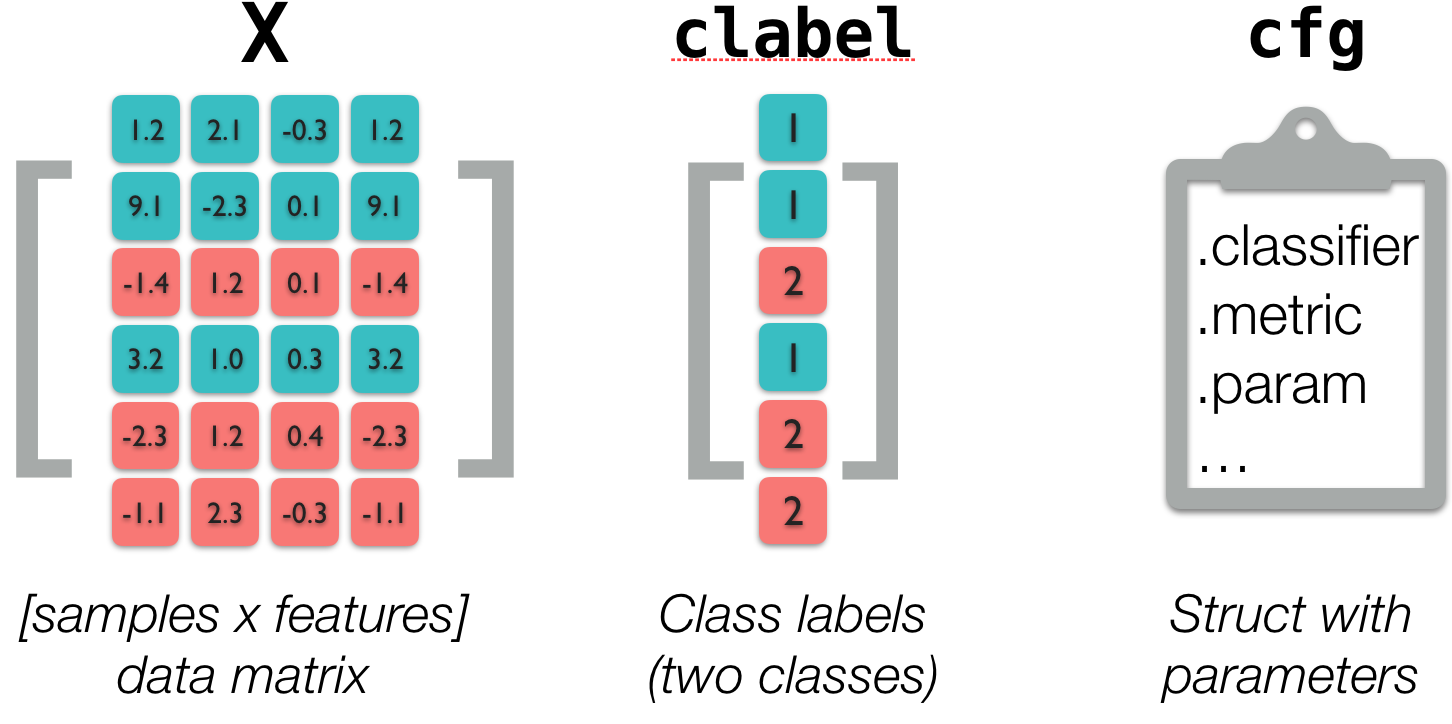
\includegraphics[width=.6\linewidth]{X_clabel_cfg}
\caption{The three most commonly used input arguments in \mvpa. Colours are used to represent the two classes 1 (turquoise) and 2 (red) for illustrative purposes. Note that \ttt{X} can be  three-dimensional (e.g. if it also has a time dimension) or higher-dimensional (e.g. time-frequency data).}
\label{fig:X}
\end{figure}

The toolbox can be interacted with easily using a set of high-level functions that cover many common classification tasks. These functions perform an entire cross-validated classification analysis given a dataset with specific dimensions and class labels. \ttt{mv\_crossvalidate} performs  cross-validation on a 2-D [samples $\times$ features] dataset \ttt{X}. The next two functions, \ttt{mv\_classify\_across\_time}  and \ttt{mv\_classify\_timextime}, assume that the data has a time dimension as well, i.e. it is a 3-D [samples $\times$ features $\times$ time points] array. \ttt{mv\_classify\_across\_time} performs classification for every time point, resulting in a vector of cross-validated metrics (e.g. accuracy), the length of the vector being the number of time points. In contrast, \ttt{mv\_classify\_timextime} performs  classification for every combination of training and test time points, resulting in a matrix of cross-validated metrics. \ttt{mv\_searchlight} takes 2-D or 3-D input data and performs classification for every feature separately, resulting in a vector of cross-validated metrics, the length of the vector being the number of features (e.g. channels). Lastly, \ttt{mv\_classify} is a more general-purpose function that works on data of arbitrary dimension (e.g. time-frequency data). It combines the capabilities of all the other high-level functions at the expense, to some extent, of ease to use and speed.

\todo{ discuss preprocess}

All high-level functions take the three input arguments depicted in \prettyref{fig:X}. First, \ttt{cfg}, a configuration structure wherein hyperparameters for the analysis can be set. Second, \ttt{X}, the input data array of appropriate dimension. Third, \ttt{clabel}, a vector of class labels.
Some of the parameters in the \ttt{cfg} struct are common  to all high-level functions:


\begin{itemize}
    \item \ttt{cfg.classifier}: specifies the classifier (default \ttt{'lda'}). Classifiers are introduced in detail in \prettyref{sec:classifiers}.
    \item \ttt{cfg.param}: a substruct that specifies the hyperparameters for the classifier. For instance, \ttt{cfg.param.lambda = 0.1} sets the hyperparameter for shrinkage regularisation in LDA.
    \item \ttt{cfg.balance}: specifies an approach to deal with imbalanced data. \ttt{cfg.balance = 'oversample'} oversamples the minority class(es) in the training set, and \ttt{'undersample'} undersamples the majority classes. Alternatively, a target number of samples per class can be specified (e.g. \ttt{cfg.balance = 50}). Undersampling and oversampling is used within each class to attain the target. As a result, all classes have the same number of samples.
    \item \ttt{cfg.replace}: if \ttt{cfg.balance} is set to \ttt{'oversample'} or \ttt{'undersample'}, replace determines whether data is drawn with replacement (default 1).
    \item \ttt{cfg.metric}: specifies the metric to be calculated from the classifier outputs. e.g. classification accuracy or AUC (default \ttt{'accuracy'}). Metrics are introduced in detail in \prettyref{sec:metrics}.
\end{itemize}

The \ttt{cfg} struct also holds the cross-validation settings explained in more detail in the next section. Regarding the \ttt{cfg.balance} parameter, it is worth noting that undersampling is performed at the level of the repeats, whereas oversampling is performed only within each training set. This is necessary because in oversampling data points are  replicated. As a result, the same data point could end up both in the training set and in the test set, leading to overfitting.

% \begin{table}
% \centering
% \footnotesize
% \begin{tabularx}{\textwidth}{|c| l X |}
%  \hline
%  Input & Type & Description \\ [0.5ex]
%  \hline\hline
%  \ttt{cfg} & struct & MATLAB structure with parameters specifying details of the analysis (e.g. classifier, cross-validation, how to deal with imbalanced data)\\
%  \ttt{X} & matrix  & EEG/MEG data matrix. Usually 2-D [samples x features] or 3-D [samples x features x time].  \\
%  \ttt{clabel} & vector & vector of class labels \\ [1ex]
%  \hline
% \end{tabularx}
% \caption{Input arguments to the high-level functions.}
% \label{table:input}
% \end{table}

\subsubsection{Cross-validation}

To obtain a realistic estimate of classifier performance and control for overfitting, a classifier should be tested on an independent dataset that has not been used for training. In most neuroimaging experiments, there is only one dataset with a restricted number of trials. K-fold cross-validation makes efficient use of this data by splitting it into k different folds. In every iteration, one of the k folds is held out and used as test set, whereas all other folds are used for training. This is repeated until every fold has been used as test set once. Since cross-validation itself is stochastic due to the random assignment of samples to folds, it can be useful to repeat the cross-validation several times and average the results. See \cite{Lemm2011} for a discussion of cross-validation and potential pitfalls. Cross-validation is implemented in all high-level functions. It is controlled by the following parameters:

\begin{itemize}
    \item \ttt{cfg.cv}: cross-validation type, either \ttt{'kfold'}, \ttt{'leaveout'} or \ttt{'holdout'} (default \ttt{'kfold'})
    \item \ttt{cfg.k}: number of folds in k-fold cross-validation (default 5)
    \item \ttt{cfg.repeat}: number of times the cross-validation is repeated with new randomly assigned folds (default 5)
    \item \ttt{cfg.p}: if \ttt{cfg.cv} is \ttt{'holdout'}, \ttt{p} is the fraction of test samples (default 0.1)
    \item \ttt{cfg.stratify}: if 1, the class proportions are approximately preserved in each test fold (default 1)
\end{itemize}


\subsubsection{Classification across time: \ttt{mv\_classify\_across\_time}}

Many neuroimaging datasets have a 3-D structure (trials x channels x time). The start of the trial (t=0) typically corresponds to stimulus or response onset. Classification across time can help identify at which time point in a trial discriminative information shows up. To this end, classification is performed across trials, for each time point separately. This is implemented in the function \ttt{mv\_classify\_across\_time}. It returns classification performance calculated for each time point in a trial.


\subsubsection{Time generalisation: \ttt{mv\_classify\_timextime}}

Classification across time does not give insight into whether information is shared across different time points. For example, is the information that the classifier uses early in a trial (t=80 ms) the same that it uses later (t=300ms)? This question can be answered by training the classifier at t=80ms and testing it at t=300ms, and vice versa. Repeating this analysis for every possible combination of training time point and testing time point yields a [training time points $\times$ testing time points] matrix of classification results. In the literature, this kind of analysis is also known as time generalisation \cite{King2014}. The function  \ttt{mv\_classify\_timextime} implements time generalisation. It returns a 2D matrix of classification performance, with performance calculated for each combination of training time point and testing time point.

\subsubsection{Searchlight analysis:  \ttt{mv\_searchlight}}

Which features contribute most to classification performance? The answer to this question can be used to to perform feature selection or to aid interpretability by localising the discriminative information in feature space. To this end, \ttt{mv\_searchlight} performs cross-validated classification for each feature separately. If there is a spatial structure in the features (e.g. neighbouring electrodes, neighbouring voxels), groups of features rather than single features can be considered. The result is a classification performance measure for each feature. If the features are e.g. channels, the result can be plotted as a topography.


\subsubsection{Classification of multi-dimensional data: \ttt{mv\_classify}}

In some cases, a dataset can have more than 3 dimensions. An obvious example is time-frequency data which is 4-dimensional, e.g. samples $\times$ channels  $\times$ frequencies $\times$ time points. Even more complex datasets using e.g. connectivity data are easily conceivable. Furthermore, it is conceivable that the user wants to analyse the data in different ways. For instance, time-frequency example, one user may want a two-dimensional classification result obtained for each time/frequency point, using the channels as features. In other cases, it may be desirable to perform a time x time analysis, using both channels and frequencies as features, or a frequency x frequency analysis, using channels and time points as features. Clearly, a more flexible function is required that works with arbitrary data dimensionality and that allows for the designation of dimensions to be treated as features, for searchlight, or for generalisation.

It is worth pointing out that \texttt{mv\_classify} is a general-purpose function that is a generalisation of \texttt{mv\_searchlight}, \texttt{mv\_classify\_across\_time}, and \texttt{mv\_classify\_timextime}. In other words, any of these functions actions can be 'simulated' using \texttt{mv\_classify}.

\todo{this function needs to be actually written}


%%% -----------------------------
%%% ------- PREPROCESSING -------
%%% -----------------------------
\subsection{Preprocessing}

\todo{implement the code, write the section}


%%% -----------------------------
%%% -------- CLASSIFIERS --------
%%% -----------------------------
\subsection{Classifiers}\label{sec:classifiers}

Classifiers are implemented using pairs of train/test functions. For instance, an LDA classifier is trained by calling

\begin{verbatim}
cf = train_lda(param, X, clabel)
\end{verbatim}

where \ttt{X} is the training data and \ttt{clabel} are the corresponding class labels. \ttt{param} is a MATLAB struct that contains hyperparameters. Hyperparameters are specific for each classifier. For instance, \ttt{param.lambda = 0.5} sets the regularisation hyperparameter in LDA to 0.5. In many cases, the default hyperparameters yield good results. However, for fine control of the hyperparameters, the user can refer to the documentation of the train functions. The hyperparameters for LDA can be accessed by typing \ttt{help(train\_lda)} in MATLAB. The output \ttt{cf} is another struct that describes the classifier. For linear classifiers, \ttt{cf.w} is the weight vector specifying the linear combination of features and \ttt{cf.b} is the threshold/bias term. After training, the classifier can be applied to test data, also denoted as \ttt{X}, by calling

\begin{verbatim}
[clabel, dval, prob] = test_lda(cf, X)
\end{verbatim}

The first output argument \ttt{clabel} is the \textit{predicted} class labels. They can be compared against the true class labels to calculate a classification performance metric. \ttt{test\_lda} provides two additional outputs, but not all classifiers have this capability. \ttt{dval} is the \textit{distance to the hyperplane/decision boundary}, a dimensionless distance measure. \ttt{prob} is a probability estimate, that is, the probability for a given sample to belong to class 1. For the time being, probablility estimate are only supported for two-class problems.

If the high-level interface is used, the train/test functions are called  automatically. In this case, all the user is required to do is to specify the classifier when calling the high-level function, e.g. \ttt{cfg.classifier = 'lda'}. If desired, hyperparameters can be passed by setting the param substructure, e.g.  e.g. \ttt{cfg.param.lambda = 0.5}.

In the following section, the individual classifiers are introduced. Whenever math is used, it is assumed that the data is contained in matrix $\X\in\R^{n \times p}$ of $n$ samples and $p$ predictors/features. The i-th row of this matrix is denoted as the column vector $\x_i\in\R^p$. For binary classification problems, it is assumed that the classes are coded as +1 and -1 and stored in a vector $\mathbf{y}\in\R^n$ with $y_i$ referring to the i-th class label.

%%% -------- LDA --------
\subsubsection{Linear Discriminant Analysis: \ttt{'lda'}, \ttt{'multiclass\_lda'}}

Two-class LDA is implemented as the classifier \ttt{'lda'} whereas multi-class LDA is implemented as \texttt{'multiclass\_lda'}. LDA operates in two separate steps \cite{Fisher1936}. In the first step, the data is mapped onto a $(C-1)$-dimensional subspace, where $C$ is the number of classes. In the second step, a sample is assigned to the class with the closest class centroid. LDA thus acts as a prototype classifier within the subspace. The coordinates for the mapping are found by iteratively solving the equation

\begin{equation}
\label{eq:fda}
\w_{\text{lda}} = \underset{\w}{\text{arg max}}\ \frac{\w^\top S_B\w}{\w^\top S_W\w}
\end{equation}

where $\S_b$ and $\S_w$ are defined as

\begin{equation*}
%\label{eq:scatter-means-multi}
\begin{alignedat}{2}
\S_b =\ & \sum_{j\,\in\{1,2,...,C\}}n_j\,(\mm{j} -\mbar) (\mm{j} - \mbar)^\top\ \quad &&\text{(between-classes scatter)}\\
\S_w =\ & \sum_{j\,\in\{1,2,...,C\}}\sum_{i\in\mathcal{C}_j} (\x_i - \mm{j})(\x_i - \mm{j})^\top\  \quad &&\text{(within-class scatter)}\\
\end{alignedat}
\end{equation*}

Here, $n_j$ is the number of instances in class $j$, $\m_j$ is the $j$-th class mean, $\mbar$ is the sample mean, and $\mathcal{C}_j$ is the set of indices of instances in class $j$. For two classes, LDA is equivalent to linear regression \cite{Treder2019DirectFDA} and, applied to event-related potential data, it is also formally equivalent to LCMV beamforming \cite{Treder2016}. It has a simple analytical solution given by

\begin{equation}
\label{eq:lda_solution}
\w_{\text{lda}} = \S_w^{-1}\ (\m_1 - \m_2)
\end{equation}

For multiple classes, there is multiple vectors $\w_{\text{lda}}$. They are collected in a matrix $\W\in\R^{P\times(C-1)}$ and scaled such that $\W^\top\S_w\W = \I$ \cite{Bishop2007}. $\W$ can be obtained via the generalised eigenvalue problem

\begin{align}
\label{eq:LDA-eigenvalue-multiclass}
\S_b\,\W = \S_w\,\W\mathbf{\Lambda}
\end{align}

where $\mathbf{\Lambda}$ is a diagonal matrix of eigenvalues.

As for binary LDA, ridge regularisation can be applied to the within-class scatter matrix by replacing $\S_w$ by $\S_w+\lambda\I$ \cite{Friedman1989}.

In EEG/MEG data, $\S_w$ is often ill-conditioned or singular and hence the inverse in \prettyref{eq:lda_solution} cannot be calculated reliably. Therefore, shrinkage regularisation is applied by default and $\S_w$ is replaced by $\widetilde{\S}_w$:

\begin{align}
\label{eq:shrinkage}
\widetilde{\S}_w = (1-\lambda_\text{shrink})\ \S_w + \lambda_\text{shrink}\,\nu\,\I
\end{align}

where $\I$ is the identity matrix and $\nu = \text{trace}(\S_w)/p$ \cite{Blankertz2011}. Shrinkage downweighs the off-diagonal elements of the scatter matrix. The regularisation hyperparameter $\lambda_\text{shrink}\in [0,1]$ blends between the unregularised covariance ($\lambda=0$) and spherical covariance ($\lambda=1$). For $\lambda=1$, LDA becomes a prototype classifier, that is, each sample is assigned to the closest centroid in feature space. By default (\ttt{param.lambda = 'auto'}), $\lambda_\text{shrink}$ is estimated automatically using the Ledoit-Wolf formula \cite{Ledoit2003HoneyMatrix,Blankertz2011}.

In the literature, LDA has also been used with ridge-regression type regularisation, yielding $\widetilde{\S}_w = \S_w + \lambda_\text{ridge}\,\I$ with $\lambda_\text{ridge}\in [0,\infty)$ \cite{Friedman1989RegularizedAnalysis}. The user can switch to ridge regularisation by setting \ttt{param.reg = 'ridge'}. However, both regularisation approaches are equivalent up to scaling. For a given $\lambda_\text{shrink}<1$, the same regularisation effect can be obtained using ridge regularisation by setting $\lambda_\text{ridge} = \nu\lambda_\text{shrink} / (1-\lambda_\text{shrink})$
\cite{Treder2018Cross-validationLDA}.


%%% -------- KERNEL FDA --------
\subsubsection{Kernel Fisher Discriminant Analysis: \ttt{'kernel\_fda'}}

Kernel Fisher Discriminant Analysis (KFDA) is the kernelised version of LDA. Roughly speaking, kernels allow for the data to be mapped into a high-dimensional space wherein LDA is performed. Since the map is non-linear, the resultant hyperplane in high-dimensional space corresponds to a non-linear decision boundary in the original feature space \todo{ref Mika and Hastie/Bishop}. This allows for the solution of non-linear classification problems.

$\mathbf{N}^{-1} \mathbf{M}$

Like in LDA, the model can be regularised using ridge regularisation (\ttt{param.reg = 'ridge'}) or shrinkage regularisation (\ttt{param.reg = 'shrink'}). Unlike LDA, there is currently no approach for automatically choosing the hyperparameter $\lambda$, so it needs to be set by the user.

\todo{finish up kernel fda}

%%% -------- LOGISTIC REGRESSION --------
\subsubsection{Logistic regression: \ttt{'logreg'}}

In Logistic Regression (LR) for two classes, the class probabilities are modelled directly by fitting a logistic function to the data \cite{Hastie2009}. Given a data point $\x$ and weights $\w$, the probability is given by

\begin{equation}
\label{eq:logreg_probability}
P(y = \pm 1\,|\,\x,\w) = \frac{1}{1 + \text{exp}(-y\,\w^\top\x)}
\end{equation}

where it is assumed that the threshold/bias is contained in the weight vector and that $\X$ has been augmented with a column of 1's. The weights $\w$ are found by minimising the logistic loss function

\begin{equation}
\label{eq:logreg_loss_function}
\L_\text{LR}(\w) = \sum_{i=1}^n \log(1 + e^{-y_i\w^\top\x_i})
\end{equation}

This optimisation problem is convex and there is only one (global) optimum. However, there exists no analytical solution. Instead, an iterative algorithm is required to optimise $\w$. In \mvpa{}, the Trust Region Newton Method introduced by Lin et al. \cite{Lin2007TrustRegression} has been implemented in the MATLAB function \ttt{TrustRegionDoglegGN}.

To counteract overfitting, the user can choose between two regularisation approaches. In log-F(1,1) regularisation (\ttt{param.reg = 'logf'}), Jeffrey's prior is imposed on the weights \cite{Firth1993BiasEstimates,Rahman2017PerformanceData.,King2001}. The regularisation is implemented via data augmentation. Alternatively, L2-regularisation can be used to impose a Gaussian prior on the weights. In this case, a penalty term is added to the loss function:

\begin{equation}
\label{eq:logreg_loss_function}
\L_\text{LR}^{L2}(\w) = \L_\text{LR}(\w) + \frac{\lambda}{2}\, ||\w||^2
\end{equation}

Here, $\lambda\in [0,\infty)$ controls the amount of regularisation. While log-F(1,1) regularisation does not require any hyperparameters, L2-regularisation requires $\lambda$ to be set. It can be set to a fixed value by the user. Alternatively, a range of candidate $\lambda$'s can be specified (e.g. \ttt{param.lambda = [0.001, 0.01, 0.1, 1]}). A nested cross-validation is then performed to select the optimal $\lambda$.
Unfortunately, this kind of hyperparameter optimisation is very costly, since the classifier has to be trained multiple times for each value of the hyperparameter. To speed up optimisation, 'warm starts' are used; in warm starts, the initial value for $\w$, denoted as  $\w_\text{init}$, is set to the solution of the previous iteration. The initialisation regime works as follows:

\begin{itemize}
    \item In iteration 1, $\w_\text{init}$ is initialised as the zero vector.
    \item In iterations 2 and 3, $\w_\text{init}$ is initialised by the previous $\w$'s ($\w_1$ and $\w_2$).
    \item In iterations 4+, if \ttt{param.predict\_regularisation\_path=1}, then $\w_\text{init}$ is initialised by a predicted value for $\w$: for the
  k-th iteration, a quadratic polynomial is fit through $\w_{k-2}$, $\w_{k-1}$ and $\w_k$ as a function of their respective $\lambda$'s. The polynomial is then evaluated at $\lambda_k$ to obtain the prediction. Simulations show that this approach substantially reduces the number of iterations required for convergence.
\end{itemize}{}

\todo{consider showing some results for the L2 optimisation}


%%% -------- SVM --------
\subsubsection{Support Vector Machine: \ttt{'svm'}}

Just like kernel FDA, a Support Vector Machine solves non-linear classification problems by implicitly projecting the data into a high-dimensional feature space using kernels.
A two-class L1-Support Vector Machine (SVM) is implemented as the classifier \ttt{'svm'}.
The optimal weights are found by minimising the constrained dual loss objective

\begin{align}
\begin{split}
\label{eq:svm_dual_loss_function}
\text{arg min}_{\al}\quad
& \frac{1}{2} \al^\top\Q\,\al - \mathbbm{1}^\top\al\\
\text{subject to}\quad  &\ \forall i: 0 \le \al_i \le c
\end{split}
\end{align}

where $\al\in\R^n$ is the dual weight vector and  $\mathbbm{1}$ is a vector of 1's. $\Q$ is the kernel matrix with the class labels absorbed, i.e. $\Q_{ij} = y_i y_j\, k(\x_i,\x_j)$, where $k$ is the kernel function, $y_i, y_j \in\{+1, -1\}$ are the class labels for the $i$-th and $j$-th sample, and the two classes are coded as +1 and -1. The optimisation of the weights is performed using the Dual Coordinate Descent
approach by Hsieh et al. \cite{Hsieh2008ASVM} implemented in the function \ttt{DualCoordinateDescent}. The regularisation hyperparameter $c$ is controlled by setting \ttt{param.c}.


Class labels and decision values are calculated. Unlike LDA and logistic regression,
there is no underlying probabilistic model that yields class probabilities.
However, a Platt approximation using an external function (\ttt{http://www.work.caltech.edu/~htlin/program/libsvm/}) can be performed to estimate
class probabilities.


%%% -------- ENSEMBLES --------
\subsubsection{Ensemble methods: \ttt{'ensemble'}}

The \ttt{ensemble} classifier implements a meta-classifier that trains dozens
or even hundreds of classifiers such as LDA. The rationale behind training a large number of classifiers is that if each classifer manages to learn slightly different aspects about the data, their joint performance can be better than the performance of any individual classifier.
In emsemble methods, these individual classifiers are called \textit{learners}. In \mvpa{}, learners are set using the \ttt{param.learner} argument. For instance, setting \ttt{param.learner = 'lda'} trains a number of LDA classifiers. To force the learners to focus on different aspects of the data, every learner sees not the whole training data but just a subset of it. \ttt{param.nsamples} controls the number or fraction of training samples that is randomly subselected, whereas \ttt{param.nfeatures} controls the number of fraction of features.
The final classifier outut is determined via the voting strategy. If \ttt{param.stragey = 'vote'}, then the class label produced by each individual learner serves as a vote. The class that receives the maximum number of votes is then selected. If \ttt{param.stragey = 'dval'}  then the raw decision values are averaged and the final decision is taken based on whether the average is positive or negative. The latter only works for two-class classification problems.

%%% ---------------------------------
%%% ----   CLASSIFIER OUTPUT     ----
%%% ---------------------------------
\subsection{Classifier output type}\label{sec:output}

For every test sample, a classifier produces raw output. This output takes either a discrete form, as a class label (e.g. '1' for class 1), or a continuous one. If it is continuous, it comes either as a \textit{decision value} or as a \textit{probability}.
In the high-level interface, the classifier output can be specified explicitly by setting \ttt{cfg.output\_type} to \ttt{'clabel'}, \ttt{'dval'}, or \ttt{'prob'}. For most cases, however, it suffices to let \mvpa{} infer the class label. Note that decision values or probabilities are not supported for multi-class problems. This is because in multi-class the classifier output can be multi-dimensional. For two classes, the probability is a number between 0 and 1 specifying the probability that a sample belongs to class 1. Decision value is an unbounded number that can be positive or negative. Its absolute value corresponds to the distance to the hyperplane.
 If the value is positive, the predicted class label is 1; if it is negative, the predicted class label is 2.

%%% ---------------------------------
%%% ----   PERFORMANCE METRICS   ----
%%% ---------------------------------
\subsection{Classifier performance metrics}\label{sec:metrics}

In most cases, the user is not interested in the raw classifier output. Rather, the quantity of interest is a performance metric that is calculated from the classifier outputs.
This metric should reflect the degree of separability between the classes. Numerous metrics have been proposed in the literature.  When using the high-level interface, the desired metric can be specified by e.g. setting \ttt{cfg.metric = 'accuracy'}. Multiple metrics can be specified by providing a cell array, e.g. \ttt{cfg.metric = \{'accuracy', 'auc'\}}. When not using the high-level interface, the metrics can be calculated by hand using the function \ttt{mv\_calculate\_performance}. In the following, the available implemented are briefly introduced. For a more thorough discussion of classification metrics, refer to  \cite{Sokolova2009ATasks}.

\begin{itemize}
    \item \ttt{'accuracy'}: Classification accuracy represents the fraction correctly predicted class labels. Accuracy is a very popular metric, but it can be misleading when the classes are very imbalanced. The value ranges from 0 to 1 where 1 means perfect separation between the classes. If all classes have equal numbers of samples, the chance level is given by 1 divided by the number of classes.
    \item \ttt{'auc'} (for two classes only): Area under the ROC curve (AUC) is an alternative to classification accuracy. It is more robust to imbalanced classes and independent of changes to the classifier threshold. It requires continuous output from the classifier (decision values or probabilities). The value ranges from 0 to 1 where 0.5 means chance-level performance and 1 means perfect separation between the classes.
    \item \ttt{'confusion'}: The confusion matrix is a $c\times c$ matrix, $c$ being the number of classes. Rows corresponds to true class labels, columns correspond to predicted class labels. Consequently, the diagonal gives the proportion of correct classification for each class, whereas all off-diagonal elements specify the misclassifications. Concretely, the (i,j)-th element gives the proportion of samples of class i that have been classified as class j. A confusion matrix is very useful for multi-class problems since it elucidates which classes are systematically mistaken for each other.
    \item \ttt{'dval'} (for two classes only): Average decision value, for each class separately.
    \item \ttt{'precision'}: the number of true positives divided by true positives plus false positives; represents the fraction of samples labelled as positive (+1) that actually belong to the positive class. For multi-class, it is calculated per class from the unnormalised confusion matrix by dividing each diagonal element by the row sum.
    \item \ttt{'recall'} : the number of true positives divided by true positives plus false negatives; represents the fraction of samples of the positive class that have actually been detected as such. For multi-class, it is calculated per class from the confusion matrix by dividing each diagonal element by the respective column sum.
    \item \ttt{'f1'} : the F1 score combines precision and recall into a single score given by the harmonic average $2*$\ttt{precision}$*$\ttt{recall} / (\ttt{precision} + \ttt{recall}).
    \item \ttt{'tval'}: for two classes, calculates the t-test statistic for the unequal sample size, equal variance case, based on decision values. This metric can be useful as a first step for a subsequent second-level analysis across participants.
    \item \ttt{'none'}: If \ttt{cfg.metric = 'none'}, then no metric is being calculated. Instead, a cell array with the raw classifier outputs for all test sets is returned.
\end{itemize}

If cross-validation is used then the metric is initially calculated for each test set in each repetition separately. It is then averaged across test sets and repetitions. Since the number of samples in a test set can vary a proportionally weighted average is used whereby larger test sets get a larger weight.

%%% -------------------------
%%% ----  EXTENDABILITY  ----
%%% -------------------------
\subsection{Extendability}\label{sec:extendability}

\subsubsection{Custom classifiers}

\mvpa{} can easily be extended with custom classifiers. To this end, the appropriate train and test functions need to be implemented. Additionally, default hyperparamaters for the classifier need to be added to the function \ttt{mv\_get\_classifier\_param}. In the appendix, it is shown how to implement a prototype classifier that assigns a sample to the closest class centroid.

\subsubsection{LIBSVM and LIBLINEAR}

LIBSVM \cite{Chang2011LIBSVM:Machines} and LIBLINEAR \cite{Fan2008} are two high-performance libraries for SVM and Logistic Regression. Due to the usage of compiled C-code, the functions are faster than classifiers programmed in MATLAB. In order to use the libraries with \mvpa{}, the user needs to follow the installation instructions on the respective websites. In particular, the C-code needs to be compiled and added to the MATLAB path. In \mvpa{}, the classifiers are denoted as \ttt{'libsvm'} and \ttt{'liblinear'}. For a description of the hyperparameters, refer to the functions  \ttt{train\_libsvm} and \ttt{train\_liblinear}.

\subsubsection{FieldTrip integration}

\mvpa{} is a stand-alone toolbox. However, for users of FieldTrip [REF] there is a FieldTrip interface \ttt{ft\_statistics\_mvpa} that provides a direct interface between FieldTrip and \mvpa{}. High-level FieldTrip statistics functions such as \ttt{ft\_timelockstatistics} ... can be used with the parameter \ttt{cfg.method = 'mvpa'} ... The analysis is then passed on ... Users are recommended to follow the tutorial on the FieldTrip website [FOOTNOTE].

%%% -------------------------
%%% ----  DEVELOPMENT    ----
%%% -------------------------
\subsection{Development}\label{sec:development}

Apart from the \ttt{main} branch intended for general use, the GitHub repository features a \ttt{devel} branch wherein new code is developed before merging into the main branch. Additionally, the branch features code that helps in maintaining the integrity of the toolbox. The \ttt{unittests/} subfolder features a unit testing framework with specific unit tests for all classifiers, optimisation algorithms, high-level functions and some of the important utility functions. The unit tests make use of both the example EEG data, random noise, and simulated data generated from functions contained in the \ttt{simulation/} subfolder. Unit testing can be triggered by executing the \ttt{run\_all\_unittests} function.

%%% -------------------------
%%% ----  BENCHMARKIN    ----
%%% -------------------------
\subsection{Benchmarking}\label{sec:benchmarking}

In this section,
MATLAB based toolboxes ...
namely Cosmovpa, Pronto, and DMLT ... IT is also compared to the Python toolbox Sci-kit learn.

- out-of-the-box accuracy : accuracy without manual tuning of the hyperparameters by the user

- speed:

As dataset ... we used



%%%%%%%%%%%%%%%%%%%%%%%%%%%%%%%%%%%%%%%%%%%%%%%%%%%%%%
%%% -------- HYPERPARAMETER OPTIMISATION --------   %%
%%%%%%%%%%%%%%%%%%%%%%%%%%%%%%%%%%%%%%%%%%%%%%%%%%%%%%
\subsection{Hyperparameter optimisation}


...
Hyperparameters are often nuisance parameters ... It is usually not clear a priori how to set them, but their exact value ... has a substantial effect

The perhaps most common approach is nested cross-validation, whereby a set of candidate hyperparameters is tested

MVPA-Light supports hyperparameter optimisation using cross-validation. However, computationally more

\subsubsection{Regularisation hyperparameters}

recently, gradient-based methods allow for ... more efficient

...



%%%%%%%%%%%%%%%%%%%%%%%%%%%%%%%%%%%%%%%%%%%%%%%
%%% -------- REGULARISATION PATHS --------   %%
%%%%%%%%%%%%%%%%%%%%%%%%%%%%%%%%%%%%%%%%%%%%%%%
\subsection{Fast regularisation paths}


Cross-validation … a search grid … The set of classifier weights as a function of the hyperparameter(s) is also known as regularisation path
Unfortunately, manual search … is very computationally costly … since the classifier needs to be re-trained for every value or combination of values of the hyperparameter(s). To speed up this process, … computational tricks for speed-up

\subsubsection{Regularisation path for LDA}
Use Automatic estimation
Grid search: LDA involves inversion of the regularised covariance matrix. There is no cheap way to update the covariance matrix in this regularisation regime. Instead, MVPA-Light goes the following route: the data is first mapped into principal component space. The advantage here is that the covariance matrix is then diagonal and inverting a diagonal matrix is very simple... In particular the operation $C^-1$ p simply becomes $(1./D) .* p$ where $D_i = (1-lambda) sigma_i + lambda * nu$ are the regularised diagonal elements of C in PC space and $sigma_i$ is the i-th eigenvalue of C.
Simulation: compare path with and without PCA

\subsubsection{Regularisation path for logistic regression}

... warm start with the following parameters ... In the first iteration, $\w_0 = (\m_1 - \m_2)$, the vector connecting the class means. Set of $\lambda$'s $\{\lambda_1, \lambda_2, ...\}$ and a start vector $\w_0$

\begin{itemize}
\item $\lambda_1$-iteration: Set $\w_0\leftarrow \m_1 - \m_2$, where $\m_1$ and $\m_2$ are the class means.
\item $\lambda_2$ and $\lambda_3$ iterations: Set $\w_0\leftarrow \w_1$ resp. $\w_0\leftarrow \w_2$.
\item $\lambda_k$ iteration (k$>$3): Fit a quadratic polynomial $p(\lambda)$ through the points $\{(\lambda_{k-1},\w_{k-1}), (\lambda_{k-2},\w_{k-2}), (\lambda_{k-3},\w_{k-3})\}$. Set $\w_0 \leftarrow p(\lambda_k)$.
\end{itemize}

\subsubsection{Regularisation path for SVM}
Use Hastie et al procedure for estimating the full regularisation path


%%% --------- BENCHMARKING ---------
\subsection{Benchmarking experiments}


%%% --------- APPENDIX ---------
\section{Appendix}

\subsection{Implementing a prototype classifier}

This section illustrates how to implement a custom classifier. A prototype classifier assigns a new sample to the class with the closest class centroid. Class centroids are calculated from the training data by calculating the means of the samples within each class. This example is solely didactic. A prototype classifier can be simulated with LDA or multi-class LDA when setting \ttt{cfg.reg = 'shrink'} and \ttt{cfg.lambda = 1}.

First, the train function needs to be implemented. As input arguments, train functions  take a  struct of hyperparameters \ttt{param},  the training data \ttt{X} and the corresponding  class labels \ttt{clabel}. For brevity, most of the documentation is omitted.

\begin{verbatim}
    function cf = train_prototype(param,X,clabel)

    nclasses = max(clabel);

    % Classifier struct
    cf  = [];

    %% Calculate class centroids
    cf.centroid = zeros(nclasses, size(X,2));
    for c=1:nclasses
        cf.centroid(c,:) = mean(X(clabel==c,:));
    end
\end{verbatim}

The output of the train function is a structure \ttt{cf} that describes the parameter of the classifier after training. The test function takes the classifier \ttt{cf} and the test data \ttt{X} as input. We need to calculate the Euclidean distance between each test sample and each of the centroids. Then, each sample is assigned to the class whose centroid is closest.

\begin{verbatim}
    function clabel = test_prototype(cf,X)

    % Euclidean distance of each sample 
    % to each class centroid
    dist = arrayfun( @(c) sum( bsxfun(@minus, dval, ...
        cf.centroid(c,:)).^2, 2), ...
        1:cf.nclasses, 'Un',0);
    dist = cat(2, dist{:});

    % For each sample, find the closest centroid
    clabel = zeros(size(X,1),1);
    for ii=1:size(X,1)
        [~, clabel(ii)] = min(dist(ii,:));
    end

\end{verbatim}

The output of the test function is \ttt{clabel}, the vector of predicted class labels. Finally, an entry for \ttt{prototype} needs to be added to the function \ttt{mv\_get\_classifier\_param}. Since the prototype classifer has no hyperparamaters, this entry can be empty. Provided that the train and test functions are in the MATLAB path, the new classifier can be used with all high-level functions by setting \ttt{cfg.classifier = 'prototype'}.


\section*{Conflict of Interest Statement}
%All financial, commercial or other relationships that might be perceived by the academic community as representing a potential conflict of interest must be disclosed. If no such relationship exists, authors will be asked to confirm the following statement: 

The authors declare that the research was conducted in the absence of any commercial or financial relationships that could be construed as a potential conflict of interest.

\section*{Author Contributions}

MT developed the toolbox, performed all analyses and authored the manuscript.

\section*{Funding}
Details of all funding sources should be provided, including grant numbers if applicable. Please ensure to add all necessary funding information, as after publication this is no longer possible.

\section*{Acknowledgments}
I would like to thank colleagues at University of Birmingham (particularly the research groups of Bernhard Staresina, Maria Wimber, Simon Hanslmayr, and Ian Charest) and Cardiff University for early advice and adaptation of the toolbox. 
I would also like to thank Sophie Arana and Jan-Mathijs Schoffelen for their effort and advice towards integrating the toolbox in FieldTrip.

\section*{Supplemental Data}
 \href{http://home.frontiersin.org/about/author-guidelines#SupplementaryMaterial}{Supplementary Material} should be uploaded separately on submission, if there are Supplementary Figures, please include the caption in the same file as the figure. LaTeX Supplementary Material templates can be found in the Frontiers LaTeX folder.

\section*{Data Availability Statement}
The datasets [GENERATED/ANALYZED] for this study can be found in the [NAME OF REPOSITORY] [LINK]. All scripts used for this paper are available in the GitHub repository \texttt{github.com/treder/MVPA-Light-paper}.
% Please see the availability of data guidelines for more information, at https://www.frontiersin.org/about/author-guidelines#AvailabilityofData

\bibliographystyle{frontiersinSCNS_ENG_HUMS} % for Science, Engineering and Humanities and Social Sciences articles, for Humanities and Social Sciences articles please include page numbers in the in-text citations
%\bibliographystyle{frontiersinHLTH&FPHY} % for Health, Physics and Mathematics articles
\bibliography{references}

%%% Make sure to upload the bib file along with the tex file and PDF
%%% Please see the test.bib file for some examples of references

\section*{Figure captions}

%%% Please be aware that for original research articles we only permit a combined number of 15 figures and tables, one figure with multiple subfigures will count as only one figure.
%%% Use this if adding the figures directly in the mansucript, if so, please remember to also upload the files when submitting your article
%%% There is no need for adding the file termination, as long as you indicate where the file is saved. In the examples below the files (logo1.eps and logos.eps) are in the Frontiers LaTeX folder
%%% If using *.tif files convert them to .jpg or .png
%%%  NB logo1.eps is required in the path in order to correctly compile front page header %%%

\begin{figure}[h!]
\begin{center}

\includegraphics[width=10cm]{logo1}% This is a *.eps file
\end{center}
\caption{ Enter the caption for your figure here.  Repeat as  necessary for each of your figures}\label{fig:1}
\end{figure}


\begin{figure}[h!]
\begin{center}

\includegraphics[width=15cm]{logos}
\end{center}
\caption{This is a figure with sub figures, \textbf{(A)} is one logo, \textbf{(B)} is a different logo.}\label{fig:2}
\end{figure}

%%% If you are submitting a figure with subfigures please combine these into one image file with part labels integrated.
%%% If you don't add the figures in the LaTeX files, please upload them when submitting the article.
%%% Frontiers will add the figures at the end of the provisional pdf automatically
%%% The use of LaTeX coding to draw Diagrams/Figures/Structures should be avoided. They should be external callouts including graphics.

\end{document}
